\documentclass{../../../oss-apphys-exam}
\newcounter{lastmc}
\usetikzlibrary{decorations.pathmorphing,decorations.markings,calc}

\begin{document}

\gentitle{10}{ROTATIONAL MOTION, PART 2}

\raggedcolumns

\runningheader{
  \fontfamily{phv}\small
  \textcolor{gray}{AP PHYSICS C: MECHANICS $\blacksquare$}
  \textbf{MULTIPLE-CHOICE QUESTIONS}}{}{}

\begin{questions}
  \question A particle of mass $m$ moves with a constant speed $v$ at a
  distance $x_0$ parallel to the $y$-axis as shown. When the particle is in
  the position shown below, the magnitude of its angular momentum relative to
  the origin is
  \begin{center}
    \begin{tikzpicture}[scale=.9]
      \fill (2,1.5) circle (.08);
      \draw[axes] (-.2,0)--(3,0) node[right]{$x$} node[pos=0,below]{$O$};
      \draw[axes] (0,-.2)--(0,2.5) node[above]{$y$};
      \draw[thick, dashed] (0,1.5)--(2,1.5) node[pos=0,left]{$y_0$}
      --(2,0)node[below]{$x_0$};
      \draw[vectors] (2,1.5)--(2,.5) node[midway,right]{$v$};
    \end{tikzpicture}
  \end{center}
  \begin{choices}
    \choice $mvx_0$
    \choice $mvy_0$
    \choice $mv\sqrt{x_0^2+y_0^2}$
    \choice $\dfrac{mv}{\sqrt{x_0^2+y_0^2}}$
    \choice zero
  \end{choices}
    
    %\question A disk is mounted on a fixed axle. The rotational inertia of the
    %disk is $I$. The angular velocity of the disk is decreased from $\omega_i$
    %to $\omega_f$ during a time $\Delta t$ due to friction in the axle. The
    %magnitude of the average net torque acting on the wheel is
    %\begin{choices}
    %  \choice $\dfrac{\omega_f-\omega_i}{\Delta t}$
    %  \choice $\dfrac{(\omega_f-\omega_i)^2}{\Delta t}$
    %  \choice $\dfrac{I(\omega_f-\omega_i)}{\Delta t}$
    %  \choice $\dfrac{I(\omega_f-\omega_i)^2}{\Delta t}$
    %  \choice $\dfrac{I(\omega_f-\omega_i)}{\Delta t^2}$
    %\end{choices}
    %
    %\question The average power developed by the friction in the axle of the
    %disk from the previous question to bring it to a complete stop is
    %
    %\begin{oneparchoices}
    %  \choice $\dfrac{\omega_i}{\Delta t}$
    %  \choice $\dfrac{\omega_i^2}{\Delta t}$
    %  \choice $\dfrac{I\omega_i}{2\Delta t}$
    %  \choice $\dfrac{I\omega_i^2}{\Delta t}$
    %  \choice $\dfrac{I\omega_i}{\Delta t^2}$
    %\end{oneparchoices}
    %\vspace{.7in}
    %
    %\question One end of a stick of length $L$, rotational inertia $I$, and
    %mass $m$ is pivoted on an axle with negligible friction at point $P$. The
    %other end is tied to a string and held in a horizontal position. When the
    %string is cut, the stick rotates counterclockwise. The angular speed
    %$\omega$ of the stick when it reaches the bottom of its swing is
    %\cpic{.28}{end-of-stick}
    %\begin{choices}
    %  \choice $\dfrac{mgL}I$
    %  \choice $\sqrt{\dfrac{mgL}I}$
    %  \choice $\sqrt{\dfrac{2mgL}I}$
    %  \choice $\sqrt{\dfrac{mgL}{2I}}$
    %  \choice $\sqrt{\dfrac{4mgL}I}$
    %\end{choices}
    %\columnbreak
    
  \question Astronauts are conducting an experiment in a negligible gravity
  environment. Two spheres of mass $m$ are attached to either end of a light
  rod. As the rod and spheres float motionless in space, an astronaut launches
  a piece of sticky clay, also of mass $m$, toward one of the spheres so that
  the clay strikes and sticks to the sphere perpendicular to the rod. Which of
  the following statements is true of the motion of the rod, clay, and spheres
  after the collision?
  \begin{center}
    \begin{tikzpicture}
      \begin{scope}[thick]
        \draw circle(.2) node{$m$};
        \draw (0,2) circle(.2) node{$m$};
        \draw (0,.2)--(0,1.8);
        \draw (-1.2,0) circle(.2) node{$m$};
        \draw[vectors] (-1,0)--(-.5,0) node[above left]{$v$};

        \draw (1.9,0) ellipse (.35 and .2) node{$2m$};
        \draw (2,2) circle (.2) node{$m$};
        \draw (2,.2)--(2,1.8);
      \end{scope}
      \node at (0,2.5) {Before};
      \node at (2,2.5) {After};
    \end{tikzpicture}
  \end{center}
  \begin{choices}
    \choice Linear momentum is not conserved, but angular momentum is conserved.
    \choice Angular momentum is not conserved, but linear momentum is conserved.
    \choice Kinetic energy is conserved, but angular momentum is not
    conserved.
    \choice Kinetic energy is conserved, but linear momentum is not conserved.
    \choice Both linear momentum and angular momentum are conserved, but
    kinetic energy is not conserved.
  \end{choices}
  \newpage
  
  \question A rod of mass $M$, length $L$, and rotational inertia $I$ hangs
  at rest from a frictionless axle as shown. A ball of mass $m$ with a speed
  $v$ strikes the rod perpendicularly at the end of the rod. As a result
  of the collision, the ball stops. The angular speed of the rod immediately
  after the collision is
  \begin{center}
    \begin{tikzpicture}[thick]
      \fill circle (.06);
      \draw (-.15,.15) rectangle (.15,-3);
      \draw[dashed] (-.15,-.15) rectangle (3,.15);
      \draw (-2,-2.95) circle (.2) node{$m$};
      \draw[vectors] (-1.8,-2.95)--(-1,-2.95) node[midway,above]{$v$};
      \node[left] at (-.2,-1.5) {$L$};
      \node[right] at (.2,-1.5) {$I$, $M$};
    \end{tikzpicture}
  \end{center}
  \begin{choices}
    \choice $vL$
    \choice $\dfrac vL$
    \choice $\dfrac{mv}I$
    \choice $\dfrac{mv L}I$
    \choice $\dfrac{mv}{IL}$
  \end{choices}
    
%    \question A rod of mass $M$, length $L$, and rotational inertia $I$ hangs
%    at rest from a frictionless axle as shown. A ball of mass $m$ with a speed
%    $v$ strikes therod perpendicularly at the end of the rod. As a result
%    of the collision, the ball stops. The angular speed of the rod immediately
%    after the collision is
%    \begin{center}
%      \begin{tikzpicture}
%        \fill circle(.1);
%        \begin{scope}[thick]
%          \draw(.25,0) arc(0:180:.25);
%          \draw(-.25,0)--(-.25,-3);
%          \draw( .25,0)--( .25,-3);
%          \draw(-.25,-3) arc(180:360:.25);
%          \begin{scope}[dashed,rotate=90]
%            \draw(.25,0) arc(0:180:.25);
%            \draw(-.25,0)--(-.25,-3);
%            \draw( .25,0)--( .25,-3);
%            \draw(-.25,-3) arc(180:360:.25);
%          \end{scope}
%          \draw(-1,-2.8) circle(.2) node{$m$};
%          \draw[very thick,->](-1.5,-2.4)--(-.5,-2.4)
%          node[midway,above]{$v$};
%          \node[left] at (-.3,-1.5) {$L$};
%          \node[right] at (.3,-1.5) {$I$, $M$};
%        \end{scope}
%      \end{tikzpicture}
%    \end{center}
%    \begin{choices}
%      \choice $vL$
%      \choice $\dfrac vL$
%      \choice $\dfrac{mv}I$
%      \choice $\dfrac{mv L}I$
%      \choice $\dfrac{mv}{IL}$
%    \end{choices}
%    \columnbreak
    
  \uplevel{
    \textbf{Questions \ref{hollow1}--\ref{hollow2}}:
    A hollow sphere of mass $m$ and radius $R$ begins from rest at a height $h$
    and rolls down a rough inclined plane. The rotational inertia of the hollow
    sphere is $\dfrac23mR^2$.
    \begin{center}
      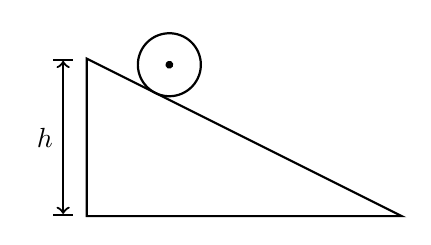
\begin{tikzpicture}[thick]
        \draw(0,0)--(-4,0)--(-4,2)--cycle;
        \draw[|<->|] (-4.3,2)--(-4.3,0) node[midway,left]{$h$};
        \begin{scope}[rotate=-atan(2/4)]
          \draw (-3.5,.4) circle (.4);
          \fill (-3.5,.4) circle (.05);
        \end{scope}
      \end{tikzpicture}
    \end{center}
  }

  \question Which of the following diagrams best represents the gravitational,
  normal and frictional forces acting on the sphere as it rolls down the plane?
  
  \begin{oneparchoices}
    \choice
    \begin{tikzpicture}[scale=.7]
      \draw circle(1);
      \fill circle(.1);
      \draw[vectors] (0,0)--(0,-2) node[below]{$F_g$};
      \draw[vectors,rotate=45] (-1,0)--(2,0) node[right]{$F_n$};
      \draw[vectors,rotate=45] (-1,0)--(-1,1.5) node[left]{$F_f$};
    \end{tikzpicture}
    \choice
    \begin{tikzpicture}[scale=.7]
      \draw circle(1);
      \fill circle(.1);
      \draw[vectors] (0,0)--(0,-2) node[below]{$F_g$};
      \draw[vectors] (0,0)--(0,2) node[above]{$F_n$};
      \draw[vectors,rotate=45] (-1,0)--(-1,1.5) node[left]{$F_f$};
    \end{tikzpicture}
    \choice
    \begin{tikzpicture}[scale=.7]
      \draw circle (1);
      \fill circle (.1);
      \draw[vectors] (0,0)--(0,-2) node[below]{$F_g$};
      \draw[vectors,rotate=45] (-1,0)--(2,0) node[right]{$F_n$};
      \draw[vectors,rotate=45] (-1,0)--(-1,-1.5) node[right]{$F_f$};
    \end{tikzpicture}
    \choice
    \begin{tikzpicture}[scale=.7]
      \draw circle (1);
      \fill circle (.1);
      \draw[vectors] (0,0)--(0,-2) node[below]{$F_g$};
      \draw[vectors,rotate=45] (-1,0)--(2,0) node[right]{$F_n$};
      \draw[vectors] (-1,0)--(-1,1.5) node[right]{$F_f$};
    \end{tikzpicture}\\      
    \choice
    \begin{tikzpicture}[scale=.7]
      \draw circle (1);
      \fill circle (.1);
      \draw[vectors,rotate=45] (0,0)--(0,-2) node[below]{$F_g$};
      \draw[vectors,rotate=45] (0,0)--(2,0) node[right]{$F_n$};
      \draw[vectors,rotate=45] (-1,0)--(-1,1.5) node[above]{$F_f$};
    \end{tikzpicture}
  \end{oneparchoices}
  \label{hollow1}
  
  \question The speed of the sphere when it reaches the bottom of the plane is

  \begin{oneparchoices}
    \choice $\sqrt{\dfrac{8gh}5}$
    \choice $\sqrt{\dfrac{6gh}5}$
    \choice $\sqrt{\dfrac{5gh}6}$
    \choice $\sqrt{\dfrac{7gh}{10}}$
    \choice $\sqrt{\dfrac{gh}2}$
  \end{oneparchoices}
  \label{hollow2}
\end{questions}
\setcounter{lastmc}{\value{question}}
\newpage
  
\runningheader{
  \fontfamily{phv}\small
  \textcolor{gray}{AP PHYSICS C: MECHANICS $\blacksquare$}
  \textbf{FREE-RESPONSE QUESTIONS}}{}{}

\begin{center}
  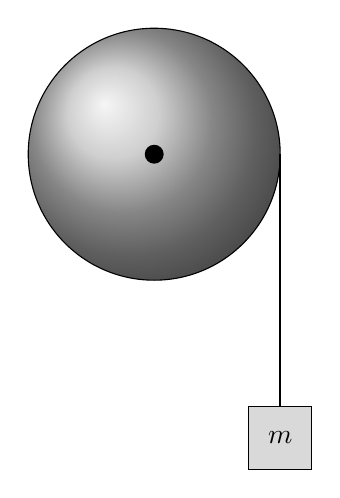
\begin{tikzpicture}[scale=.8]
    \shade[ball color=lightgray] circle (2);% node[below right]{$m$};
    \draw circle (2);
    \fill circle (.15);
    \draw[thick] (2,0)--(2,-4);
    \draw[fill=gray!30] (1.5,-4) rectangle (2.5,-5) node[midway]{$m$};
  \end{tikzpicture}
\end{center}

\begin{questions}
  \setcounter{question}{\value{lastmc}}
  \question A uniform sphere of mass $M$, and radius $R$ (rotational inertia
  $I=\dfrac25MR^2$) is free to rotate, without friction, about a horizontal axis
  through its center. A string is wrapped around the sphere and is attached to
  a body of mass $m$ as shown in the figure above.
  \begin{parts}
    \part On the diagrams below that represent the sphere and the body,
    \textbf{draw} and \textbf{label} all the forces that act on the objects.
    Forces should be drawn as arrows originating at, and pointing away from,
    the objects.
    \begin{center}
      \vspace{.4in}
      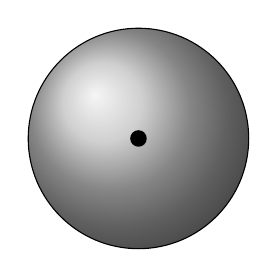
\begin{tikzpicture}[scale=.7]
        \shade[ball color=lightgray] circle (2);% node[below right]{$m$};
        \draw circle (2);
        \fill circle (.15);
      \end{tikzpicture}
      \hspace{1.75in}
      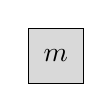
\begin{tikzpicture}[scale=.7]
        \draw[fill=gray!30] (1.5,-4) rectangle (2.5,-5) node[midway]{$m$};
      \end{tikzpicture}
      \vspace{.4in}
    \end{center}
    
    \part\textbf{Derive} an expression for the magnitude of acceleration ($a$)
    of the body.
    \vspace{\stretch1}
    
    \part\textbf{Derive} an expression for the magnitude of the tension force
    ($F_T$) in the string.
    \vspace{\stretch1}
  \end{parts}
  \newpage

  \uplevel{
    \centering
    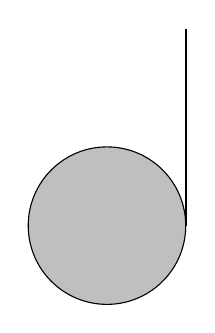
\begin{tikzpicture}[scale=.5]
      \draw[fill=lightgray] circle (2);
      \draw[thick] (2,0)--(2,5);
    \end{tikzpicture}
  }
  
  \question A cylinder of mass $M$ and radius $R$ (rotational inertia
  $I=\dfrac12MR^2$) has a string wrapped around it. The string is held fixed,
  and the cylinder falls vertically as shown in the figure above.
  \begin{parts}
    \part On the diagram that represent the cylinder, \textbf{draw} and
    \textbf{label} all forces acting on it. Forces should be drawn at the point
    where they are applied, and should be represented as arrows originating
    at, and pointing  away from, the object.
    \begin{center}
      \vspace{.7in}
      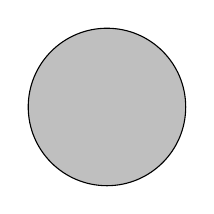
\begin{tikzpicture}[scale=.5]
        \draw[fill=lightgray] circle (2);
      \end{tikzpicture}
      \vspace{.7in}
    \end{center}
    \part\textbf{Derive} an expression for the magnitude of acceleration ($a$)
    of the body.
    \vspace{\stretch1}
    
    \part\textbf{Derive} an expression for the magnitude of the tension force
    ($F_T$) in the string.
    \vspace{\stretch1}
  \end{parts}
  \newpage


  % TAKEN FROM THE 2004 AP PHYSICS C MECHANICS EXAM FREE-RESPONSE QUESTION 2
  \uplevel{
    \centering
    \begin{tikzpicture}[scale=.85,very thick]
      \draw circle (1);
      \fill circle (.07);
      \draw (0,0)--(0,2);
      \fill[lightgray] (-3,2) rectangle (3,2.3);
      \draw (-3,2)--(3,2);
      \draw[axes,rotate=30] (0,0)--(1,0) node[midway,above]{$R$};
      \draw (-1,0)--(-1,-2);
      \draw (-1.4,-2) rectangle (-.6,-2.5) node[midway]{$m$};
      \draw[thick,|<->] (-2,-2.5)--(-2,-5) node[midway,fill=white]{$D$};
      \fill[lightgray] (-3,-5) rectangle (3,-5.3);
      \draw (-3,-5)--(3,-5);
    \end{tikzpicture}
  }
  \question A solid disk of unknown mass and known radius $R$ is used as a
  pulley in a lab experiment, as shown above. A small block of mass $m$ is
  attached to a string, the other end of which is attached to the pulley and
  wrapped around it several times. The block of mass $m$ is released from rest
  and takes a time $t$ to fall the distance $D$ to the floor.
  \begin{parts}
    \part\textbf{Determine} the magnitude of linear acceleration $a$ of the
    falling block in terms of the given quantities.
    \vspace{\stretch1}

    \uplevel{
      The time $t$ is measured for various heights $D$ and the data are
      recorded in the following table.
      \begin{center}
        \begin{tabular}{|c|c|}
          \hline
          $D$ [\si\metre] & $t$ [\si\second]\\\hline
          0.5 & 0.68 \\\hline
          1   & 1.02 \\\hline
          1.5 & 1.19 \\\hline
          2   & 1.38 \\\hline
        \end{tabular}
      \end{center}
    }
    
    \part What quantities should be graphed in order to best determine the
    acceleration of the block? \textbf{Explain} your reasoning.
    \vspace{\stretch1}

    \newpage
    \part On the grid below, \textbf{plot} the quantities determined in part
    \textbf{B}, and \textbf{label} the axes.
    \begin{center}
      \vspace{.2in}
      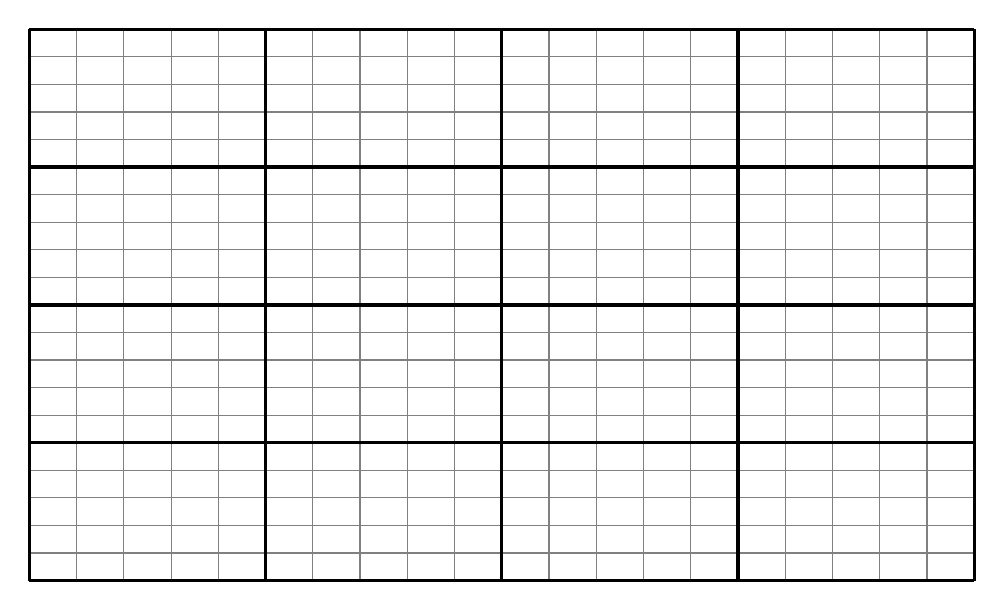
\begin{tikzpicture}[xscale=.6,yscale=.35]
        \draw[gray] grid (20,20);
        \draw[very thick,step=5] grid (20,20);
      \end{tikzpicture}
      \vspace{.2in}
    \end{center}
    \part\textbf{Draw} the best-fit line to the data.
    
    \part Use your graph above to \textbf{calculate} the magnitude of
    acceleration $a$.
    \vspace{\stretch1}

    \part\textbf{Calculate} the rotational inertia of the pulley in terms of
    $m$, $R$, $a$, and fundamental constants, as appropriate.
    \vspace{\stretch1}
    
    \part The value of acceleration found in part \textbf{E}, along with
    numerical values for the given quantities and your answer to part \text{D},
    can be used to determine the rotational inertia of the pulley. The pulley
    is removed from its support and its rotational inertia is found to be
    greater than this value. Give one \textbf{explanation} for this discrepancy.
    \vspace{\stretch2}
  \end{parts}
  \newpage

  \uplevel{
    \centering
    \begin{tikzpicture}
      \draw[very thick] (0,0)--(5,0);
      \draw[very thick, postaction=decorate,decoration={markings,
          mark= between positions 1cm and 3cm step 5mm with {
            % Places five of them
            \node[transform shape,inner sep=1pt] 
            (mark-\pgfkeysvalueof{/pgf/decoration/mark info/sequence number}) {};
          }
        }
      ]{
        decorate[
          decoration={random steps,segment length=1.5mm,amplitude=1pt}]
        %Roughness is amplitude
        {
          (5,0)--(12,0)
        }
      };

      \begin{scope}[line width=2]
        \draw (1.5,1) circle (1) node[above=30]{Sliding only};
        \draw[dashed] (6.5,1) circle (1) node[above=30]{Sliding and rotating};
        \draw[dashed] (10.5,1) circle (1) node[above=30]{Rotating, no sliding};
      \end{scope}
      \draw[axes] (1.5,1)--+(1.7,0) node[above]{$v_0$};
      \draw[axes] (6.5,1)--+(1.7,0);
      \draw[axes] (10.5,1)--+(1.7,0);
      \draw[thick,|<->|] (0,-1.3)--+(5,0) node[midway,fill=white]{No friction}
      node[below]{$t=0$};
      \draw[thick,<->|] (5,-1.3)--+(7,0) node[midway,fill=white]{
        Friction with coefficient $\mu$};
      \draw[thick,|<->|] (5,-.7)--+(4.5,0) node[midway,fill=white]{$L$};
    \end{tikzpicture}
  }
  
  \question A ring of mass $M$, radius $R$, and rotational inertia $MR^2$ is
  initially sliding on a frictionless surface at constant velocity $v_0$ to the
  right, as shown above. At time $t=0$ it encounters a surface with coefficient
  of friction $\mu$ and begins sliding and rotating. After traveling a distance
  $L$, the ring begins rolling without sliding. Express all answers to the
  following in terms of $M$, $R$, $v_0$, $\mu$, and fundamental constants, as
  appropriate.
  \begin{parts}
    \part Starting from the second law of motion in either translational or
    rotational form, as appropriate, \textbf{derive}, but do NOT solve, a
    differential equation that can be used to solve for the magnitude of the
    following as the ring is sliding and rotating:
    \begin{subparts}
      \subpart The linear velocity $v$ of the ring as a function of time $t$
      \subpart The angular velocity $\omega$ of the ring as a function of time
      $t$
    \end{subparts}
    \vspace{\stretch1}

    \part\textbf{Derive} an expression for the magnitude of the following as
    the ring is sliding and rotating.
    \begin{subparts}
      \subpart The linear velocity $v$ of the ring as a function of time $t$
      \subpart The angular velocity $\omega$ of the ring as a function of time
      $t$
    \end{subparts}
    \vspace{\stretch1}

    \part\textbf{Derive} an expression for the time it takes the ring to travel
    the distance $L$.
    \vspace{\stretch1}
    \newpage

    \part\textbf{Derive} an expression for the magnitude of the velocity of the
    ring immediately after it has travelled the distance $L$.
    \vspace{\stretch1}
    
    \part\textbf{Derive} an expression for the distance $L$.
    \vspace{\stretch2}
  \end{parts}
\end{questions}
\end{document}
